\chapter{ワークC データ取得・分析}

\section{はじめに} 
%本ワークにおいて，何を目的にどのような実験を行ったのか，得られた結果から何が考察できるのかについて報告する内容を整理して記述する．
%例えば次のように記述する．\\

%（例）本ワークでは～を目的とし，～の実験を行った．
%実験を通じて～の結果を得た．
%それらの結果より，～であることを明らかにする．

私たちが普段利用する測定機器は，物理量を数値化する測定機能と測定結果を出力する表示機能を備えている．
また，スマートフォンなどの外部コンピュータと連携し，データの記録や分析を行う通信機能を持つことがある．
本ワークでは，測定機器が持つこれらの機能のうち，出力部および通信部の開発を通じて，データを取得・分析する方法を学ぶことを目的とする．
具体的には，まずマイコンボードArduino UNO R4 WiFiに搭載されたLEDマトリクスに，センサで取得したデータを表示するプログラムを開発する．
次に，マイコンボードをWebサーバとして機能させ，測定データをネットワーク経由で外部のクライアント側PCへ送信し，グラフを作成する．
これらの開発と評価を通して，開発したプログラムの有用性を明らかにし，
測定機器におけるデータの取得と表示，および通信を介したデータの送受信と分析までの一連の流れについて理解する．

\section{方法} 
%本ワークで行った実験に関する条件や学んだ理論について記述する．
%以下の内容が記載されているか注意しながら進めること．
%例文は不慣れな学生向けの一例にすぎず，必ずしも同様の書き方をする必要はない．
%必要に応じて図表や数式を用いて説明することが求められる．

%\begin{itemize} 
%    \item[・] 実験に用いた材料およびその性能，型式など\ （例）○○の評価では，○○（型式: ○○），○○（型式: ○○），および○○（型式: ○○）を図〇〇に示すように使用した． 
%    \item[・] データの取得方法および作業手順\ （例）○○データの取得のため，○○を用いて○○を測定した．まず〇〇秒間〇〇し，次に〇〇し$\cdots$，最後に〇〇した． 
%    \item[・] 評価方法\ （例）取得されたデータを〇〇法により〇〇し，〇〇を評価した． \end{itemize}

%以下のように記述する．

%（例）本ワークでは$\cdots$を目的に$\cdots$を行った．
%○○の評価では，光センサとして○○と，○○，および○○を図〇〇に示すように配線した．
%また，○○の評価のため，○○を行った．○○のデータ取得のため，まず〇〇秒間〇〇し，次に〇〇し$\cdots$最後に〇〇した．
%取得されたデータを〇〇法により〇〇し，〇〇を評価した．

\subsection{ワークC-1 LEDマトリクスの活用}
本実習では，Arduinoに搭載された8$\times$12のLEDマトリクスを用いて，センサが取得した電圧値を表示するシステムを開発した．
この配列をmatrix.renderBitmap()関数に渡すことで，LEDマトリクスに任意のパターンを描画した．
ArduinoのanalogRead()関数で得られるデジタル値(0～1023)は，式(\ref{eq:電圧値})を用いて電圧値(0～5 V)へ変換した．
\begin{equation}
  \text{電圧値} = \frac{\text{A0ピンのデジタル値}}{1023.0} \times 5.0 \label{eq:電圧値}
\end{equation}
この電圧値を小数第2位までLEDマトリクスに表示させた．
表示させる内容は，8行12列のbyte型2次元配列で定義し，値が1の要素に対応するLEDが点灯する．
LEDマトリクスの表示例を図\ref{fig:C-1-LEDex}に示す．
\begin{figure}[H]
  \centering
  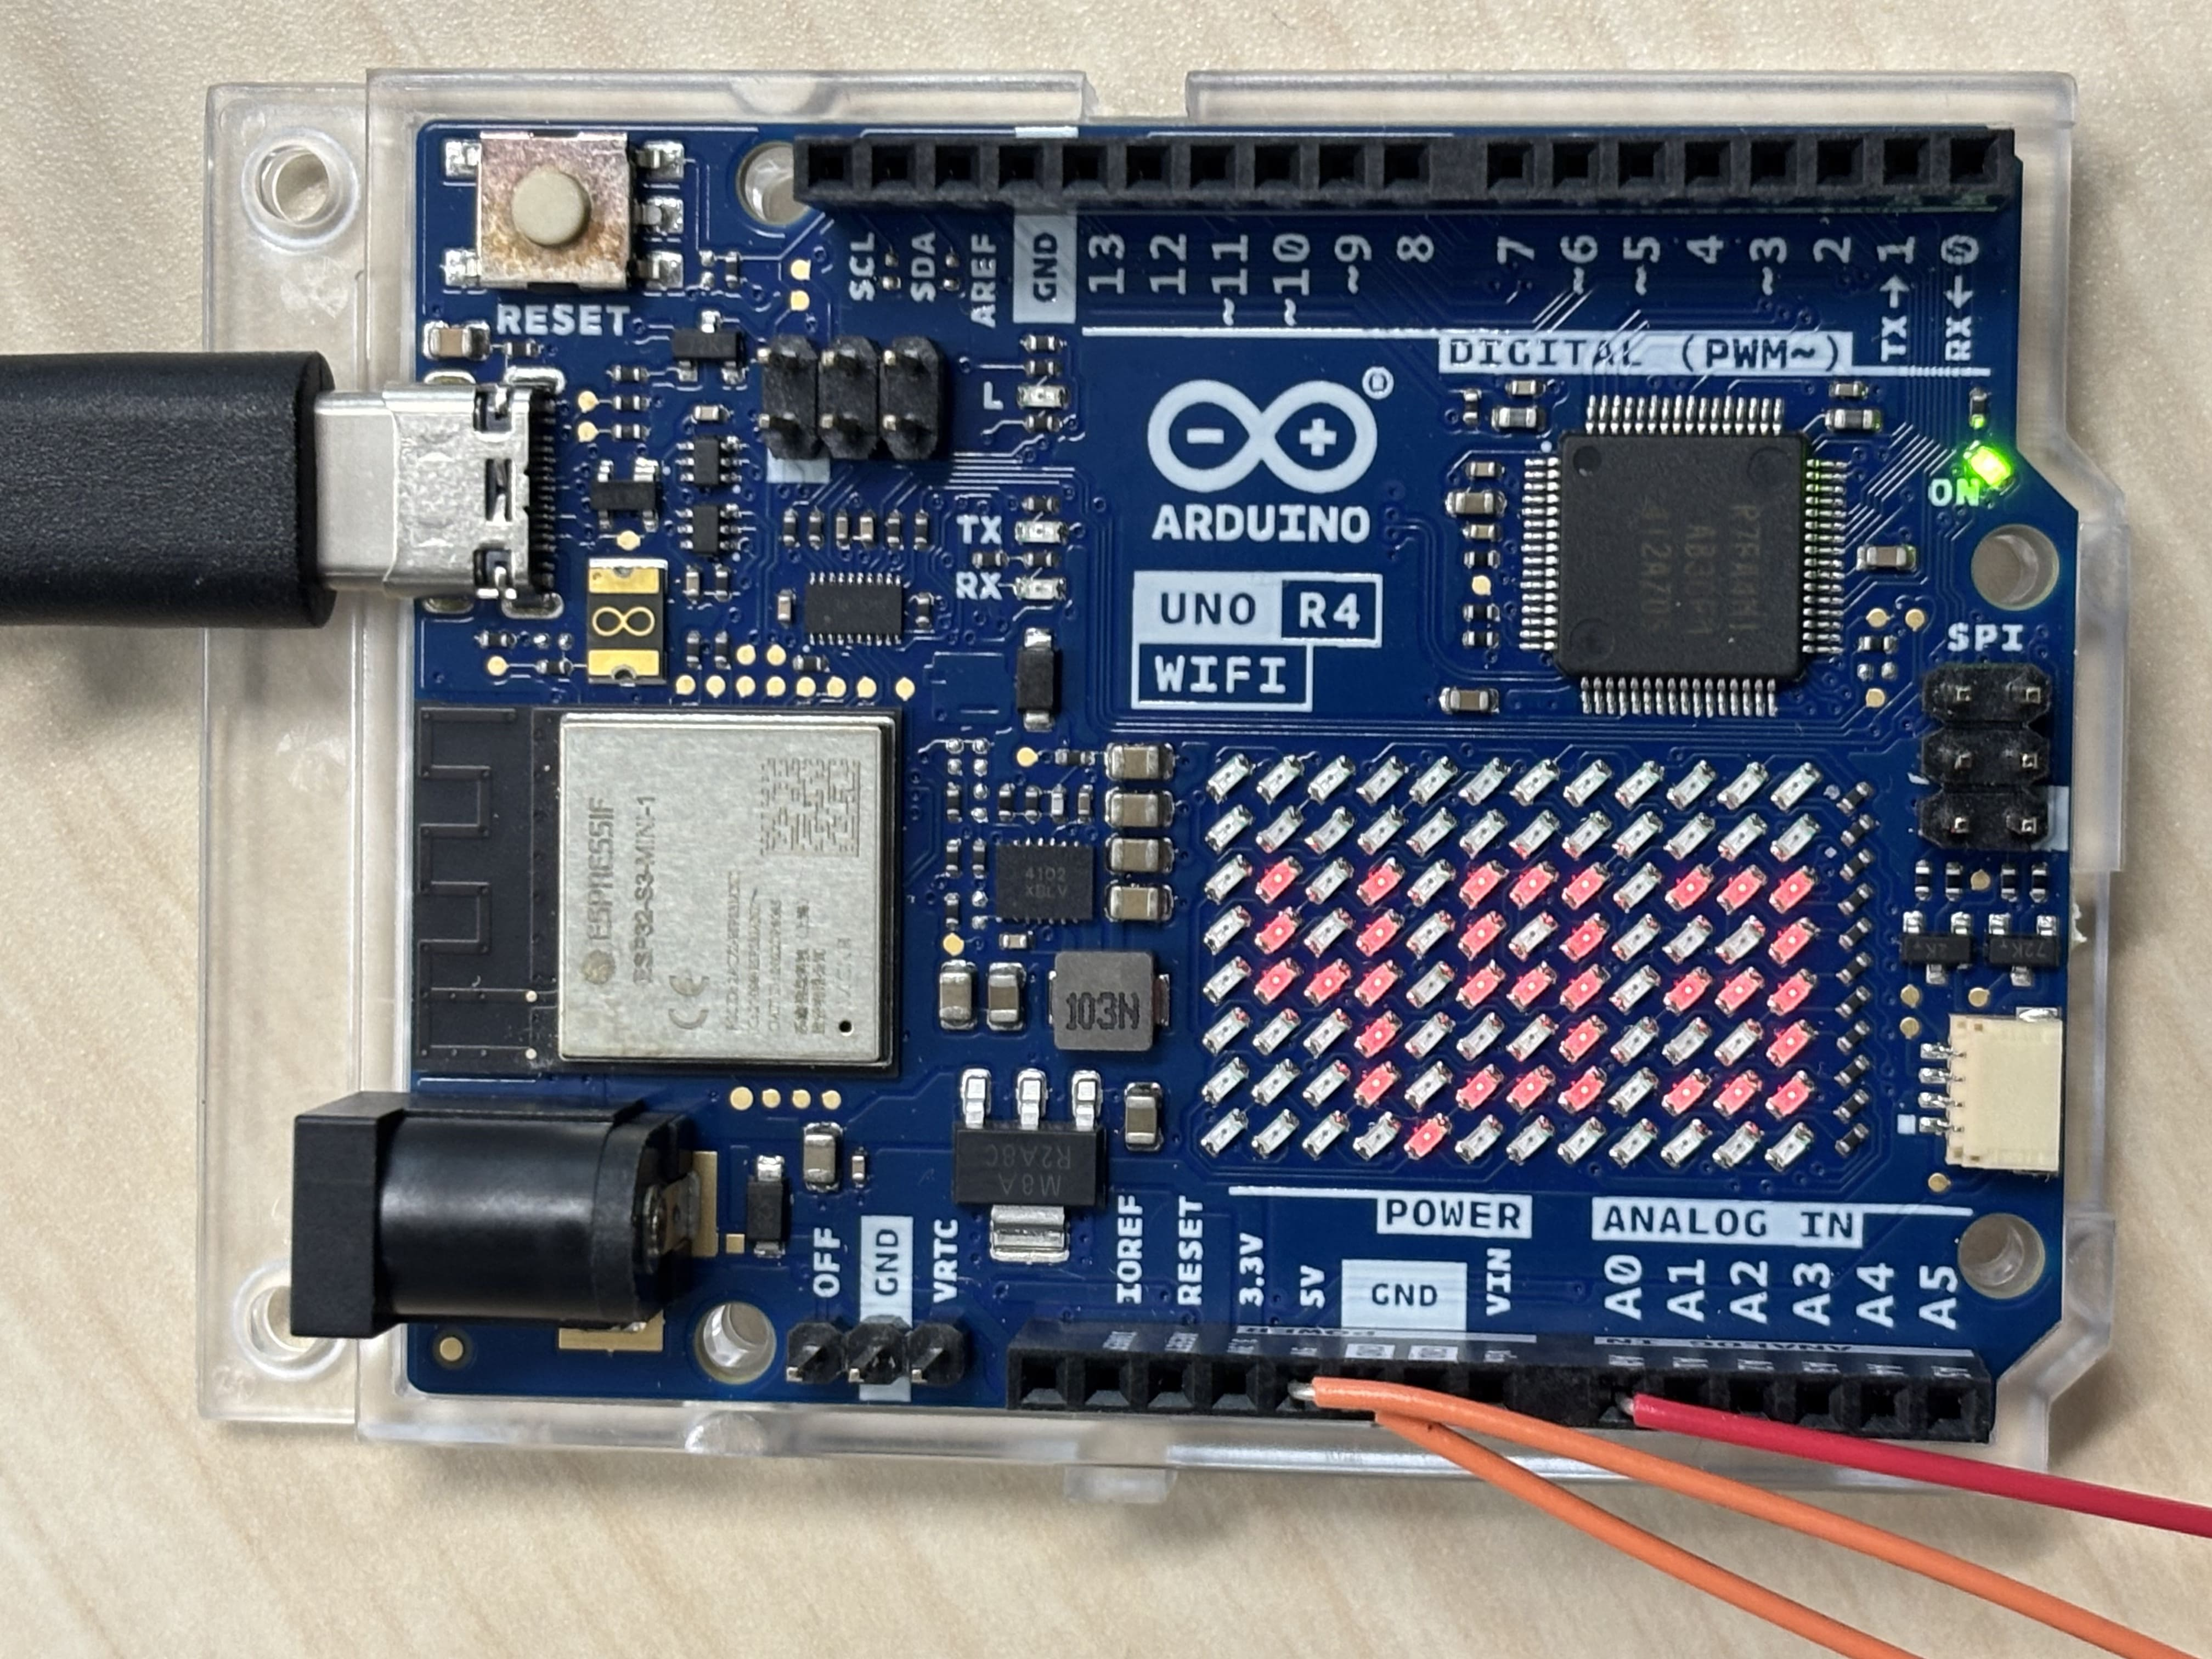
\includegraphics[width=0.8\linewidth]{fig_work_C/IMG_9242.jpg}
  \caption{電圧値を表示しているLEDマトリクスの例}
  \label{fig:C-1-LEDex}
\end{figure}

実験手順について説明する．まず，回路図を図\ref{fig:C-1-kairozu}に，実装した配線を図\ref{fig:C-1-kairo}に，使用した実験部品を表\ref{tab:C-1-1}に示す．
\begin{figure}[H]
  \centering
  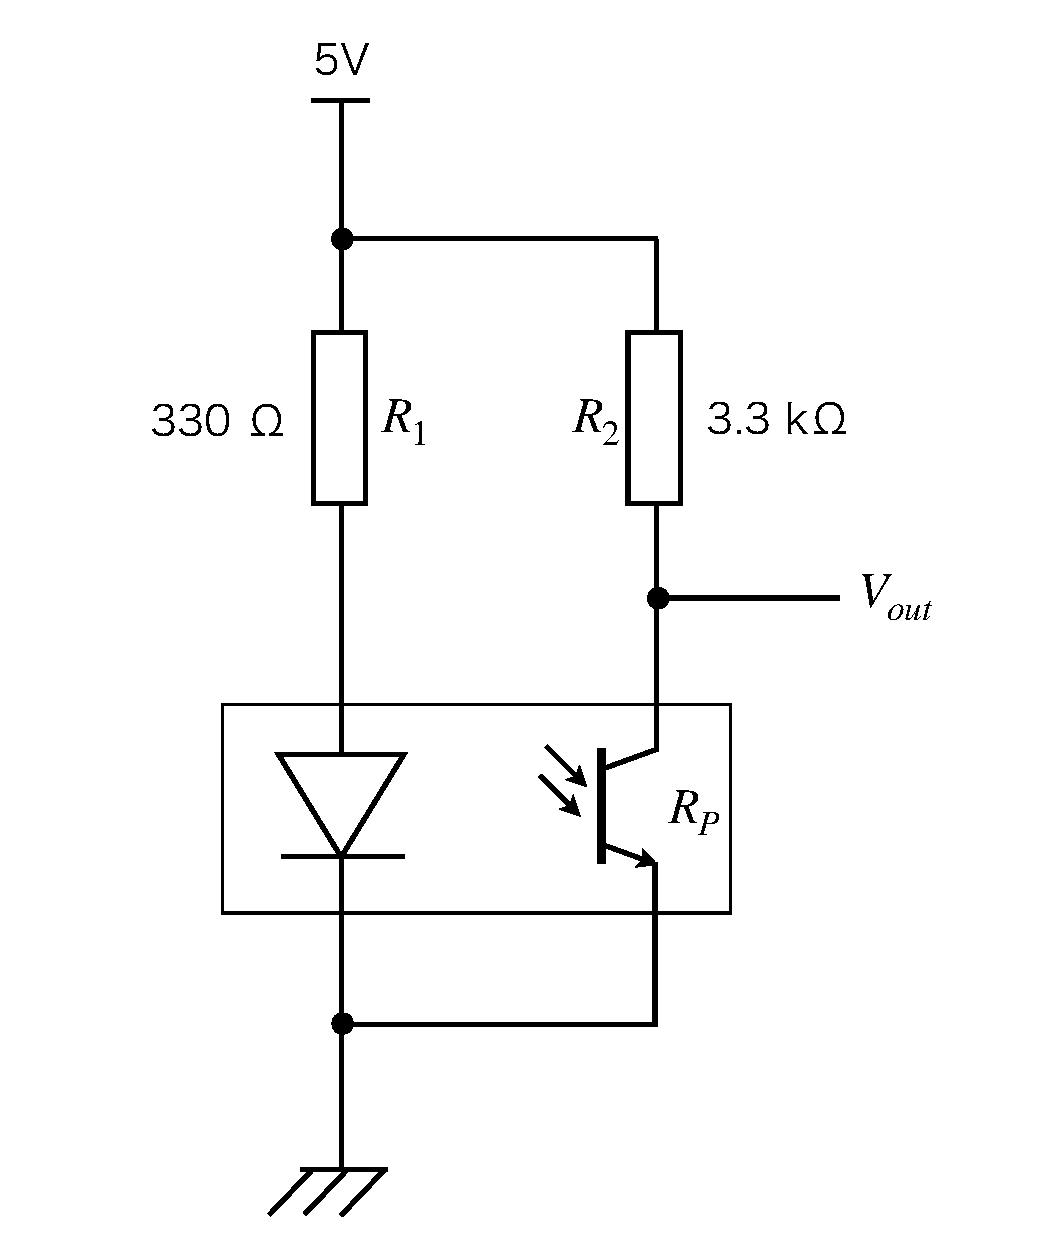
\includegraphics[width=0.7\linewidth]{fig_work_C/work_C-1_kairozu.pdf}
  \caption{フォトリフレクタを用いた分圧回路図}
  \label{fig:C-1-kairozu}
\end{figure}
\begin{figure}[H]
  \centering
  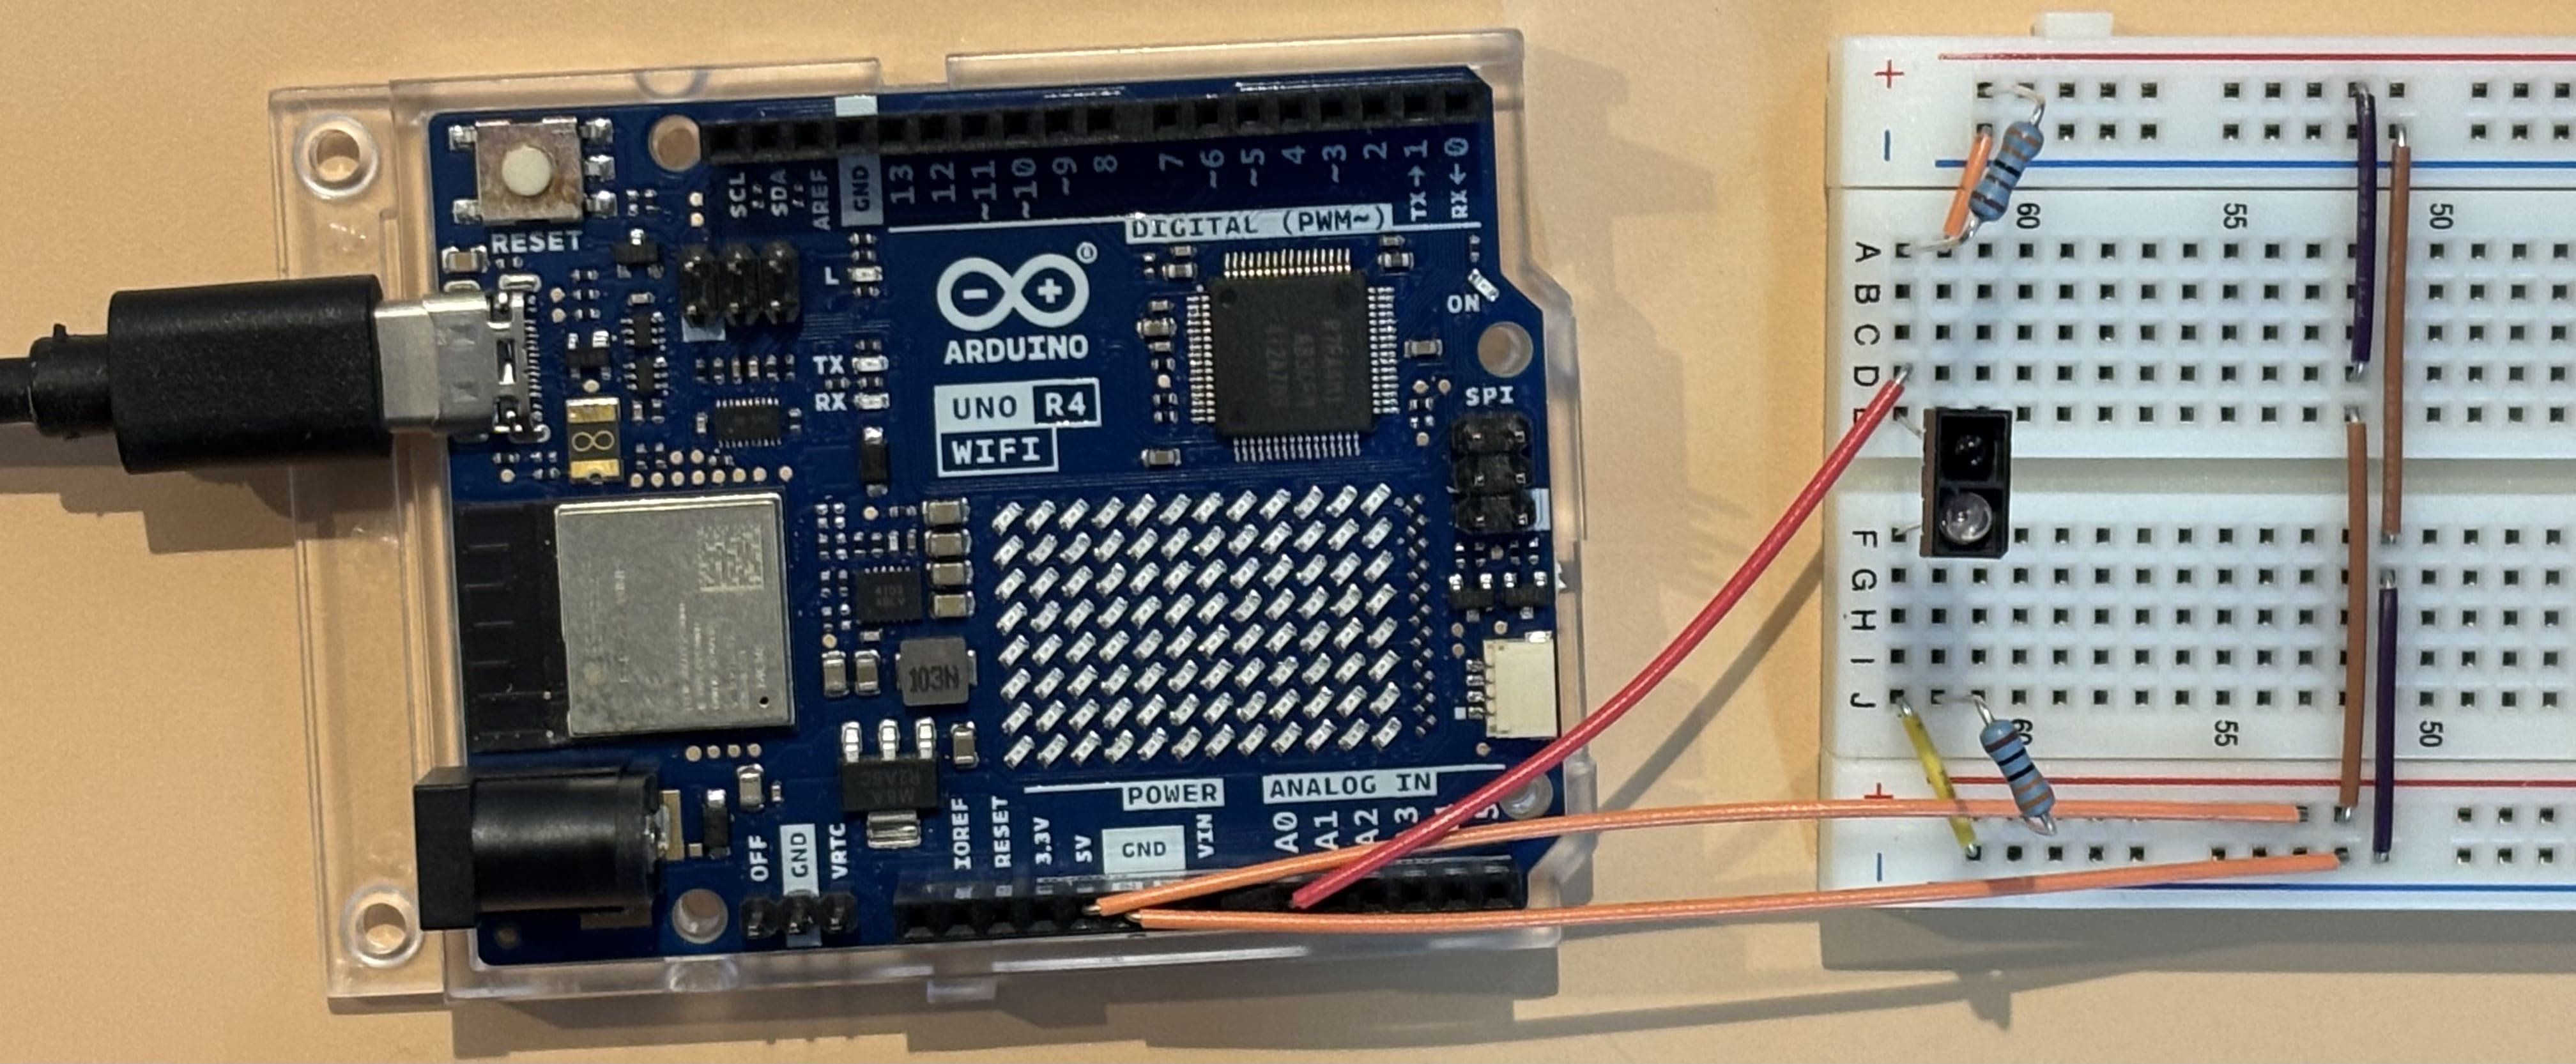
\includegraphics[width=0.9\linewidth]{fig_work_C/IMG_9240.jpg}
  \caption{フォトリフレクタを用いた分圧回路の配線}
  \label{fig:C-1-kairo}
\end{figure}
\begin{table}[H]
  \caption{使用した実験部品}
  \centering
  \begin{tabular}{|c|l|}
    \hline
    部品名 & 説明・備考 \\
    \hline \hline
    \multirow{2}{*}{Arduino Uno R4 WiFi} & A0ピンで3.3 k$\Omega$の抵抗器とフォトトランジスタの間の \\
     & アナログ値($V_{out}$)を読み取り，LEDマトリクスに結果を表示 \\
    \hline
    フォトリフレクタ & \multirow{2}{*}{遮蔽物からの反射光を検出し，距離に応じた電圧信号を出力} \\
    (LBR-127HLD)\cite{LBR-127HLD} & \\
    \hline
    抵抗器$R_1$(330 $\Omega$) & フォトリフレクタの赤外線LEDに接続する電流制限用の抵抗 \\
    \hline
    抵抗器$R_2$(3.3 k$\Omega$) & フォトリフレクタのフォトトランジスタに接続する抵抗 \\
    \hline
    ブレッドボード & 回路を実装するための土台 \\
    \hline
    ジャンパーワイヤ & Arduinoとブレッドボード，部品間の配線に使用 \\
    \hline
    PC(MacBook Pro) & 電源として使用 \\
    \hline
    USB Type-C & PCとArduinoを接続 \\
    \hline
  \end{tabular}
  \label{tab:C-1-1}
\end{table}
次に，フォトリフレクタと遮蔽物との距離を0.5 cmから5.0 cmまで0.5 cm間隔で変化させ，その際のA0ピンの電圧を測定した．
測定する際，距離を測るために定規を使用した．その計測の様子を図\ref{fig:C-1-keisoku}に示す．
\begin{figure}[H]
  \centering
  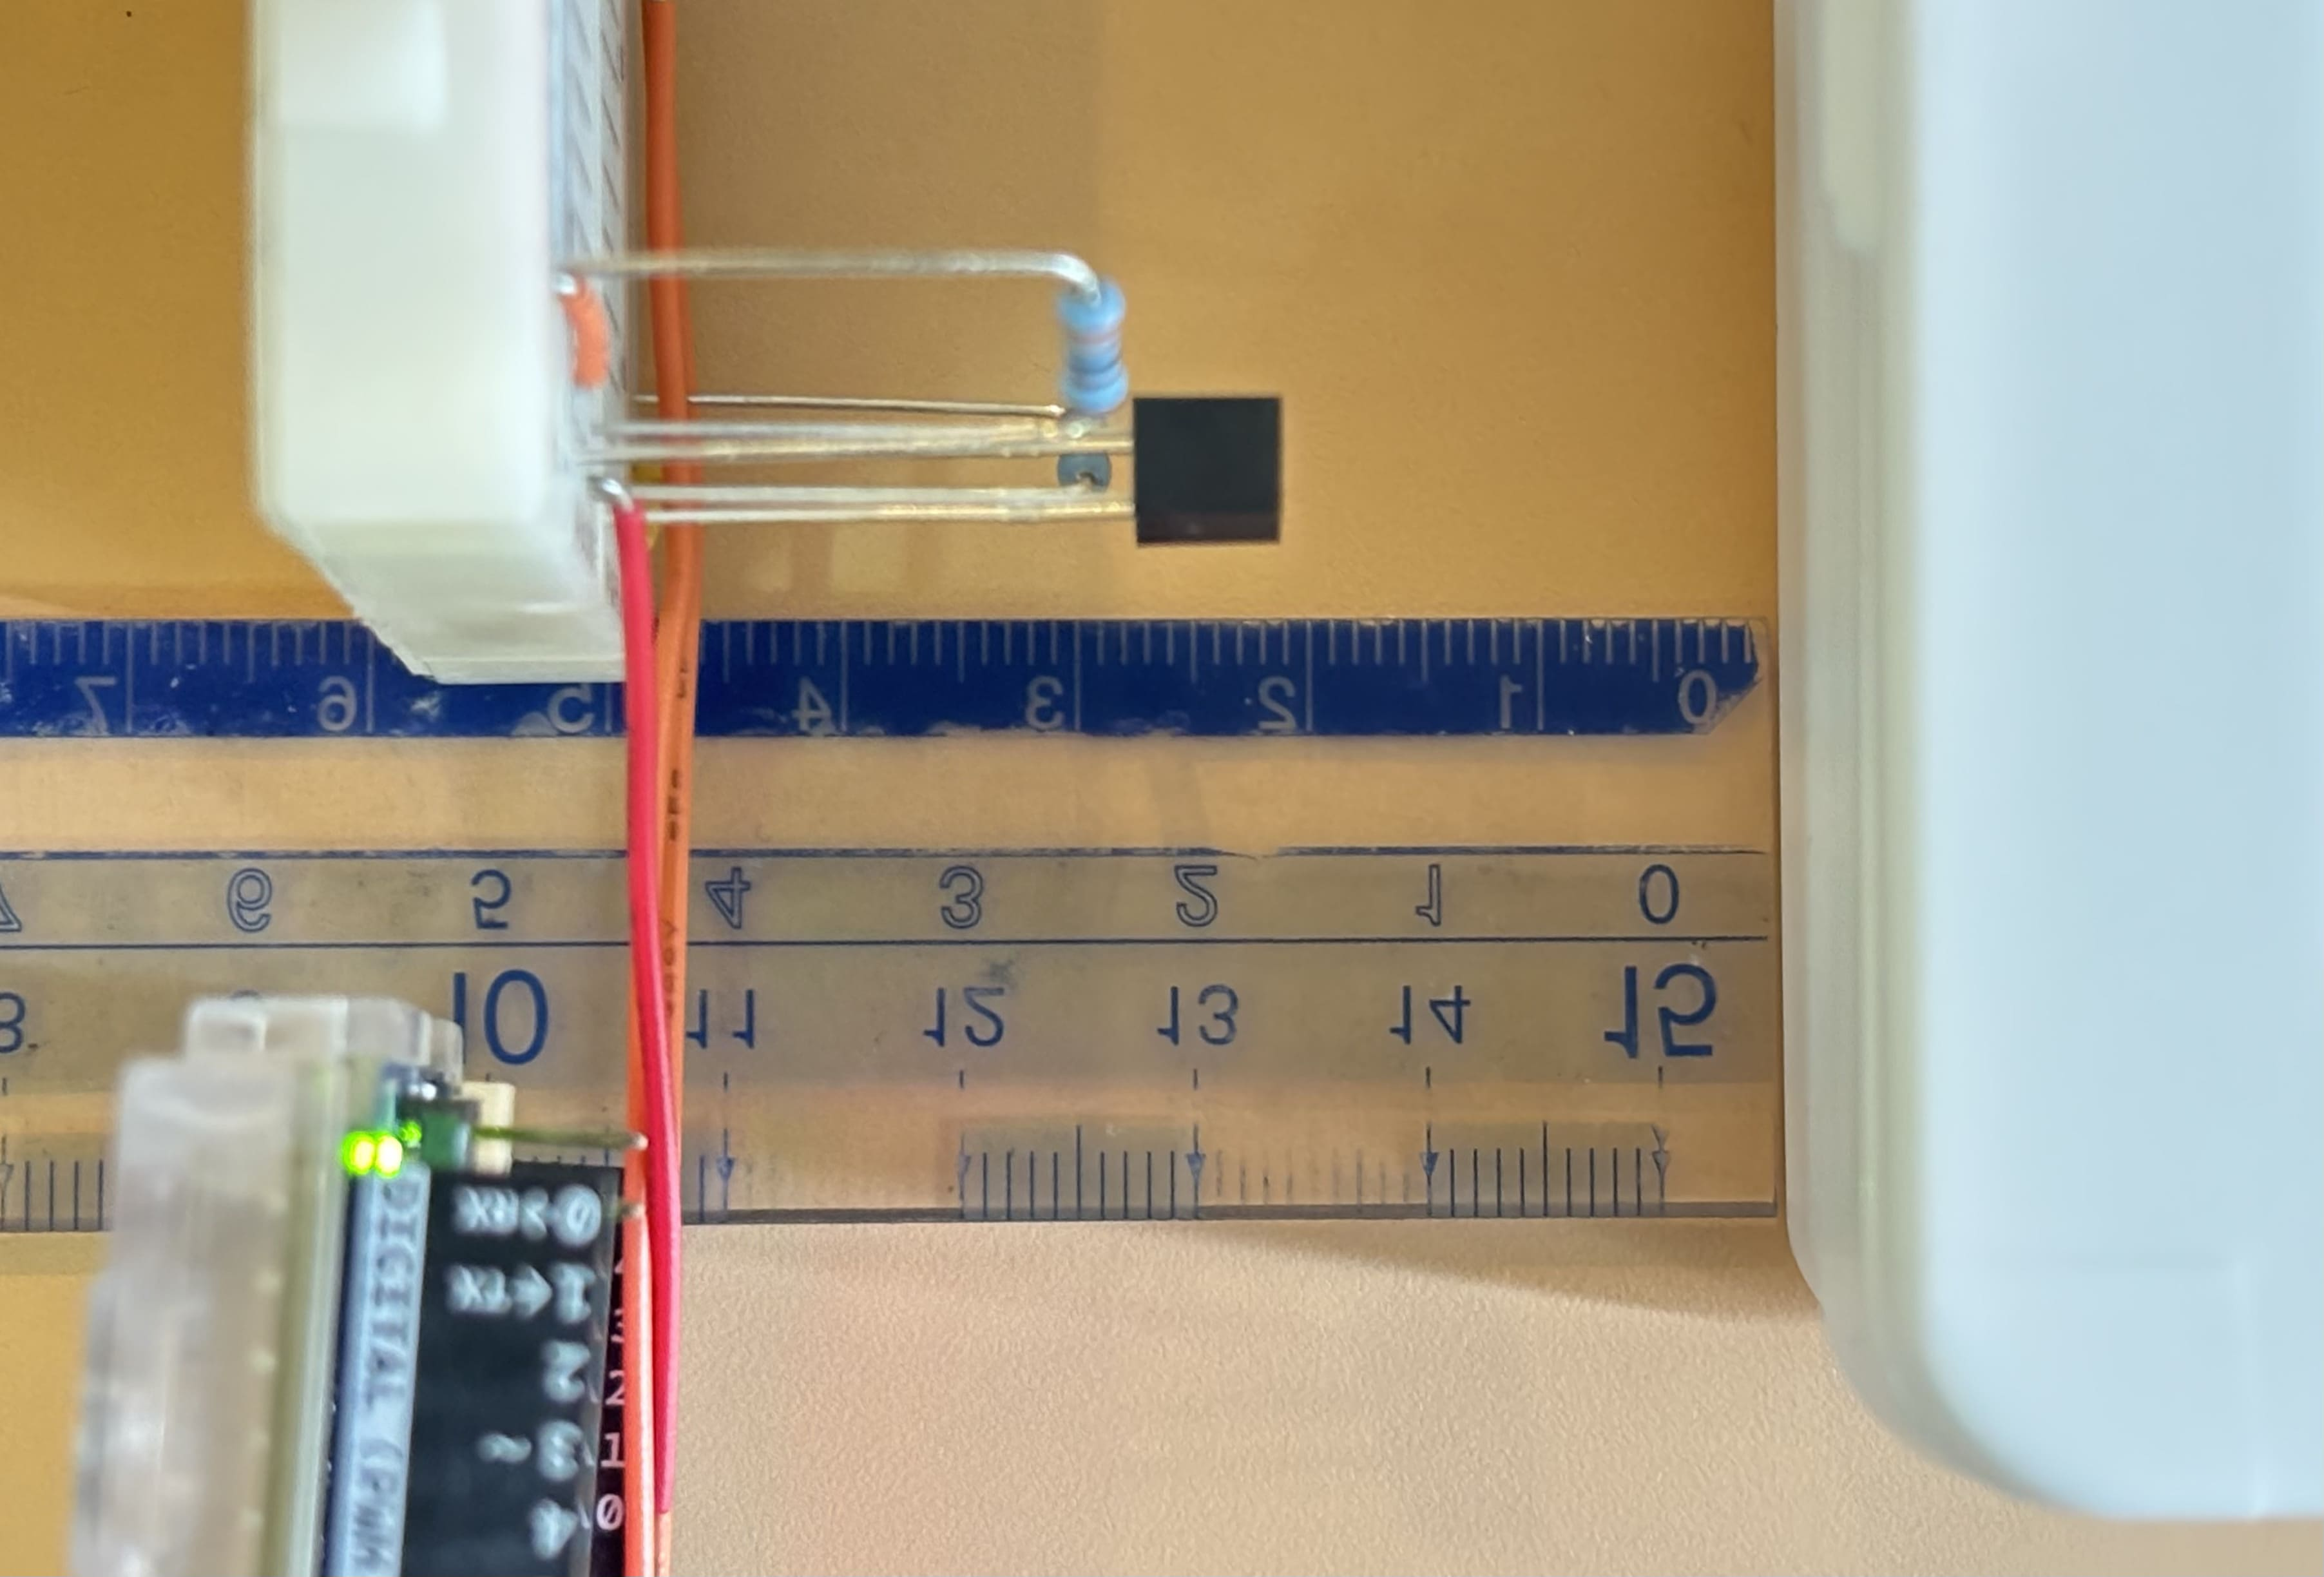
\includegraphics[width=0.9\linewidth]{fig_work_C/IMG_9238.jpg}
  \caption{フォトリフレクタと遮蔽物との距離の計測に定規を使用する様子}
  \label{fig:C-1-keisoku}
\end{figure}
測定した電圧値は遮蔽物との距離ごとに記録し，Pythonを用いて作成したフォトリフレクタと遮蔽物との距離と電圧値の関係を示すグラフで評価した．



\subsection{ワークC-2 ネットワークを介したデータの取得と分析}


本実習では，ArduinoをWebサーバとして機能させ，ネットワーク経由で測定データを取得するシステムを構築した．
ArduinoはWi-Fiモジュール(ESP32-S3)を利用してアクセスポイントモードで起動し，クライアントからのHTTPリクエスト待機状態にする．
クライアント側PCがPythonプログラムを用いてHTTP GETリクエストを送信すると，ArduinoはA0ピンで読み取った電圧値を返送する．
CdSセルは入射する光量によって抵抗値が増減するため\cite{workC_CdSセル}，この増減による電圧の変化を測定した．

回路図を図\ref{fig:C-2-kairozu}に，実装した配線を図\ref{fig:C-2-kairo}に，使用した実験部品を表\ref{tab:C-2-1}に示す．
\begin{figure}[H]
  \centering
  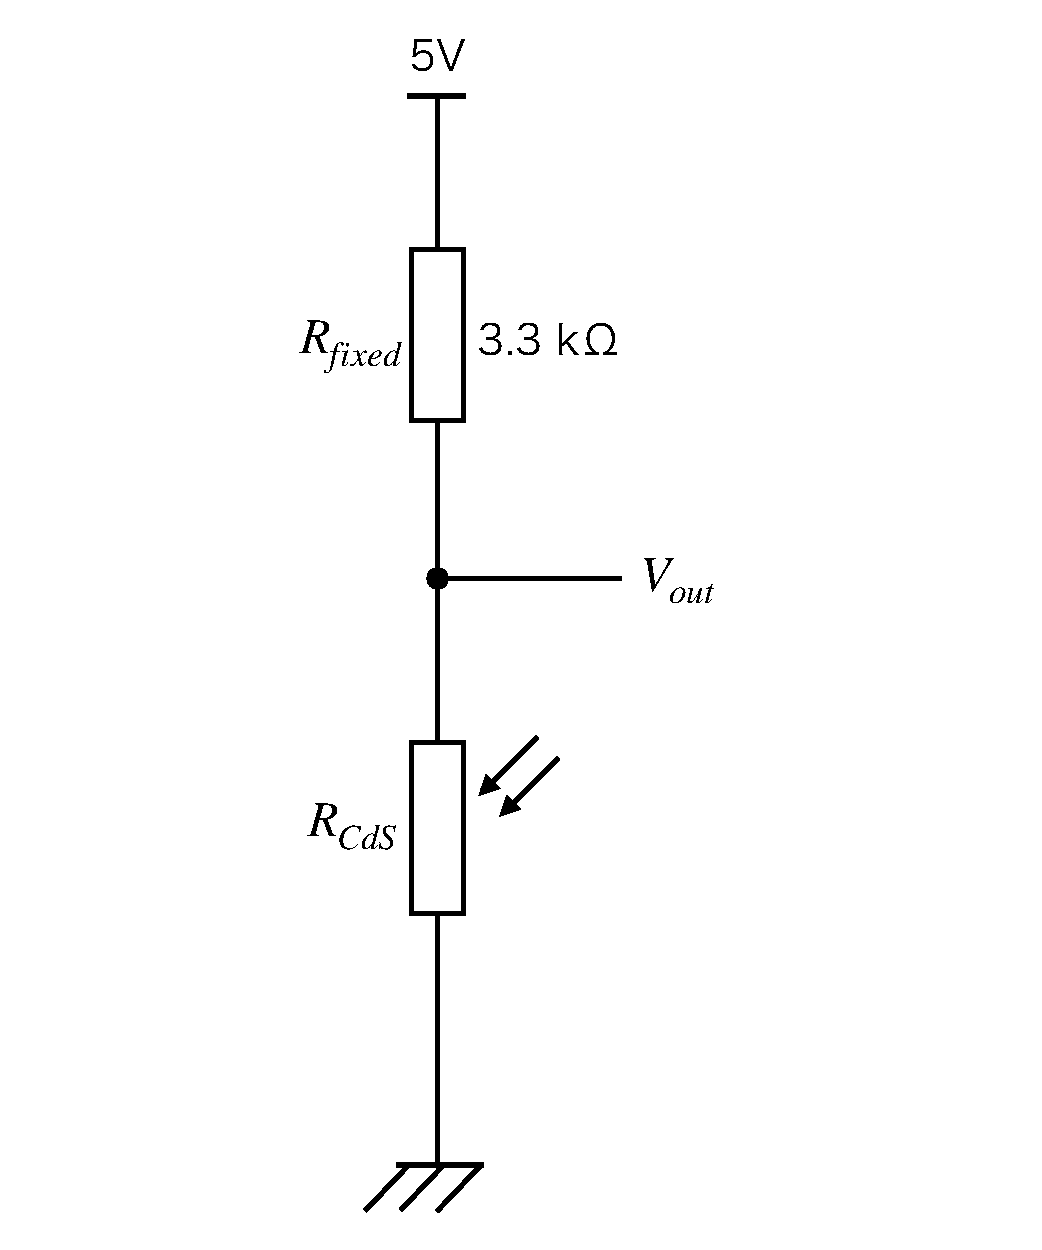
\includegraphics[width=0.7\linewidth]{fig_work_C/work_C-2_kairozu.pdf}
  \caption{CdSセルを用いた分圧回路図}
  \label{fig:C-2-kairozu}
\end{figure}
\begin{figure}[H]
  \centering
  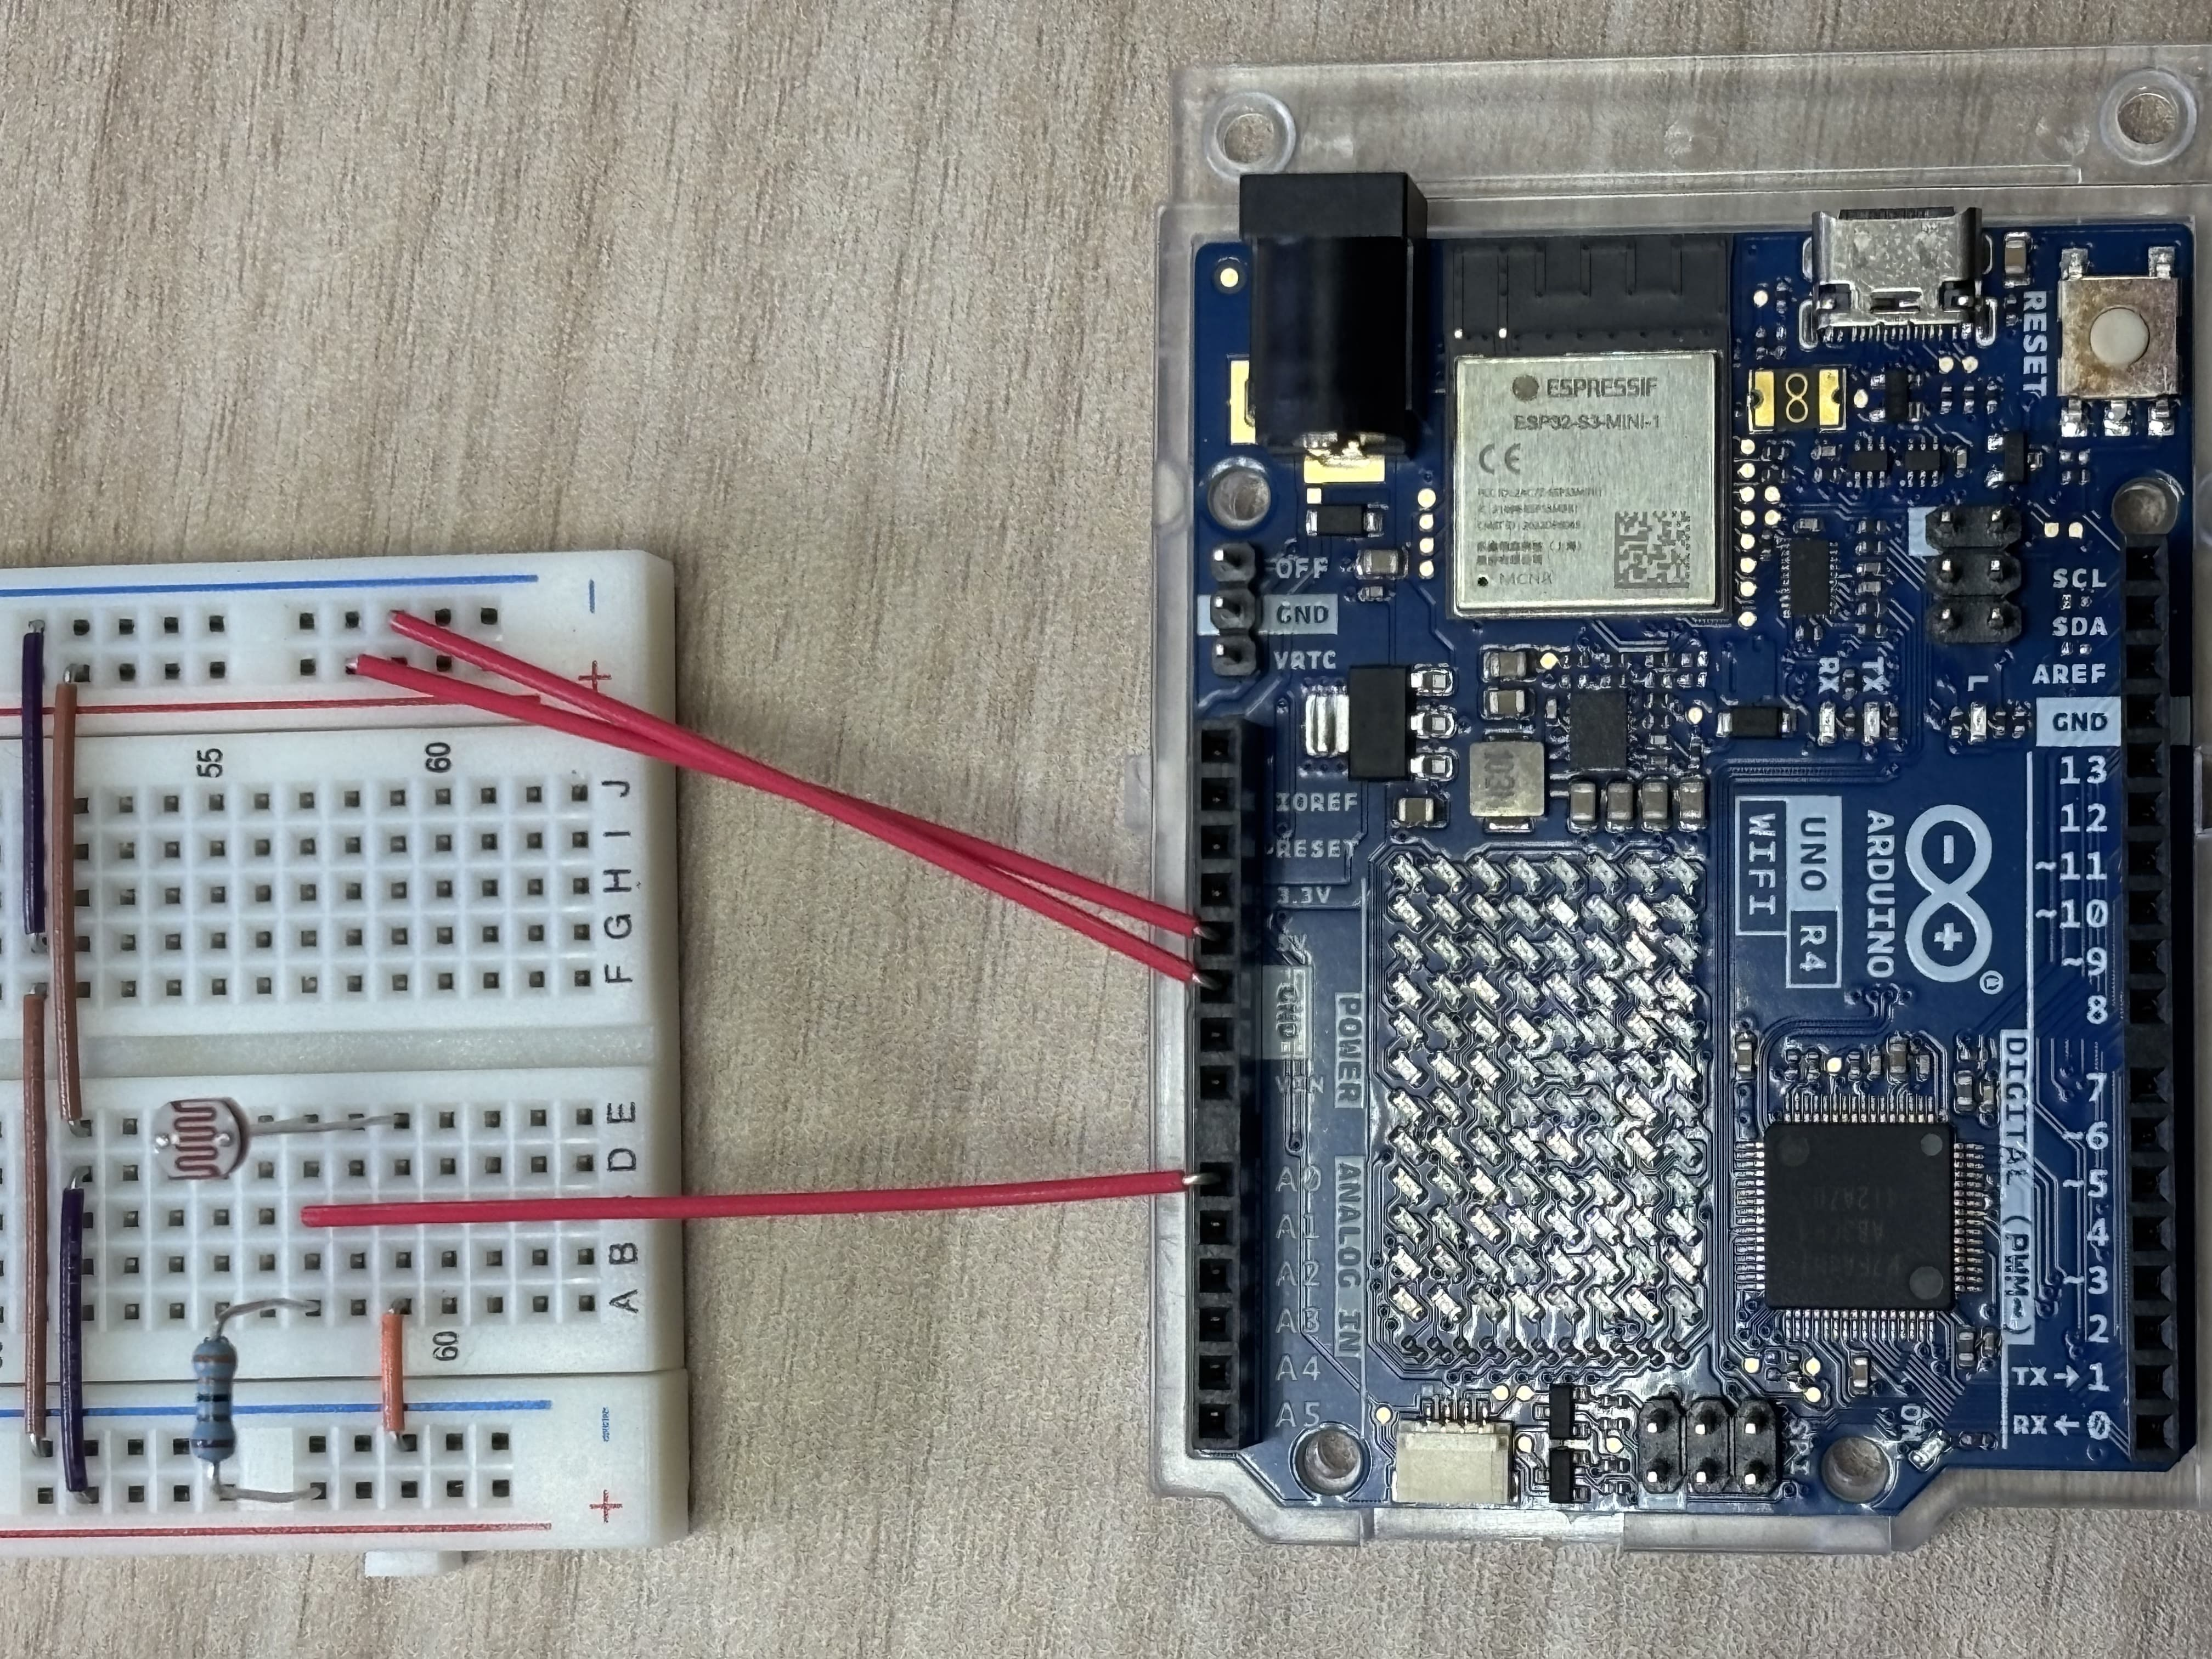
\includegraphics[width=0.8\linewidth]{fig_work_C/IMG_9271.jpg}
  \caption{CdSセルを用いた分圧回路の配線}
  \label{fig:C-2-kairo}
\end{figure}
\begin{table}[H]
  \caption{使用した実験部品}
  \centering
  \begin{tabular}{|c|l|}
    \hline
    部品名 & 説明・備考 \\
    \hline \hline
    \multirow{2}{*}{Arduino Uno R4 WiFi} & Webサーバとして機能し，A0ピンで電圧($V_{out}$)を \\
     & 測定してクライアント側PCへ送信 \\
    \hline
    CdSセル$R_{CdS}$ & \multirow{2}{*}{光の強度に応じて抵抗値が変化する光センサ} \\
    (GL3516)\cite{workC_GL3516} & \\
    \hline
    抵抗器$R_{fixed}$(3.3 k$\Omega$) & CdSセルと直列に接続し，分圧回路を構成するための抵抗 \\
    \hline
    ブレッドボード & 回路を実装するための土台 \\
    \hline
    ジャンパーワイヤ & Arduinoとブレッドボード，部品間の配線に使用 \\
    \hline
    クライアント側PC & Arduinoへリクエストを送信し，データを取得・記録 \\
    \hline
    USB Type-C & PCとArduinoを接続し，Arduinoに電力を供給 \\
    \hline
  \end{tabular}
  \label{tab:C-2-1}
\end{table}
\clearpage
実験手順として，以下の5つの条件で各20秒間ずつ電圧値を連続して測定した．
\begin{enumerate}
  \item センサ上部に何もない状態(天井の照明を受光)
  \item センサ上部約9.0 cmに手をかざした状態
  \item センサ上部約6.0 cmに手をかざした状態
  \item センサ上部約3.0 cmに手をかざした状態
  \item 再びセンサ上部に何もない状態
\end{enumerate}
クライアント側PCからは1秒ごとにリクエストを送信し，取得したデータを時系列データとしてCSVファイルに記録した．
その計測の様子を図\ref{fig:C-2-keisoku}に示す．
\begin{figure}[H]
  \centering
  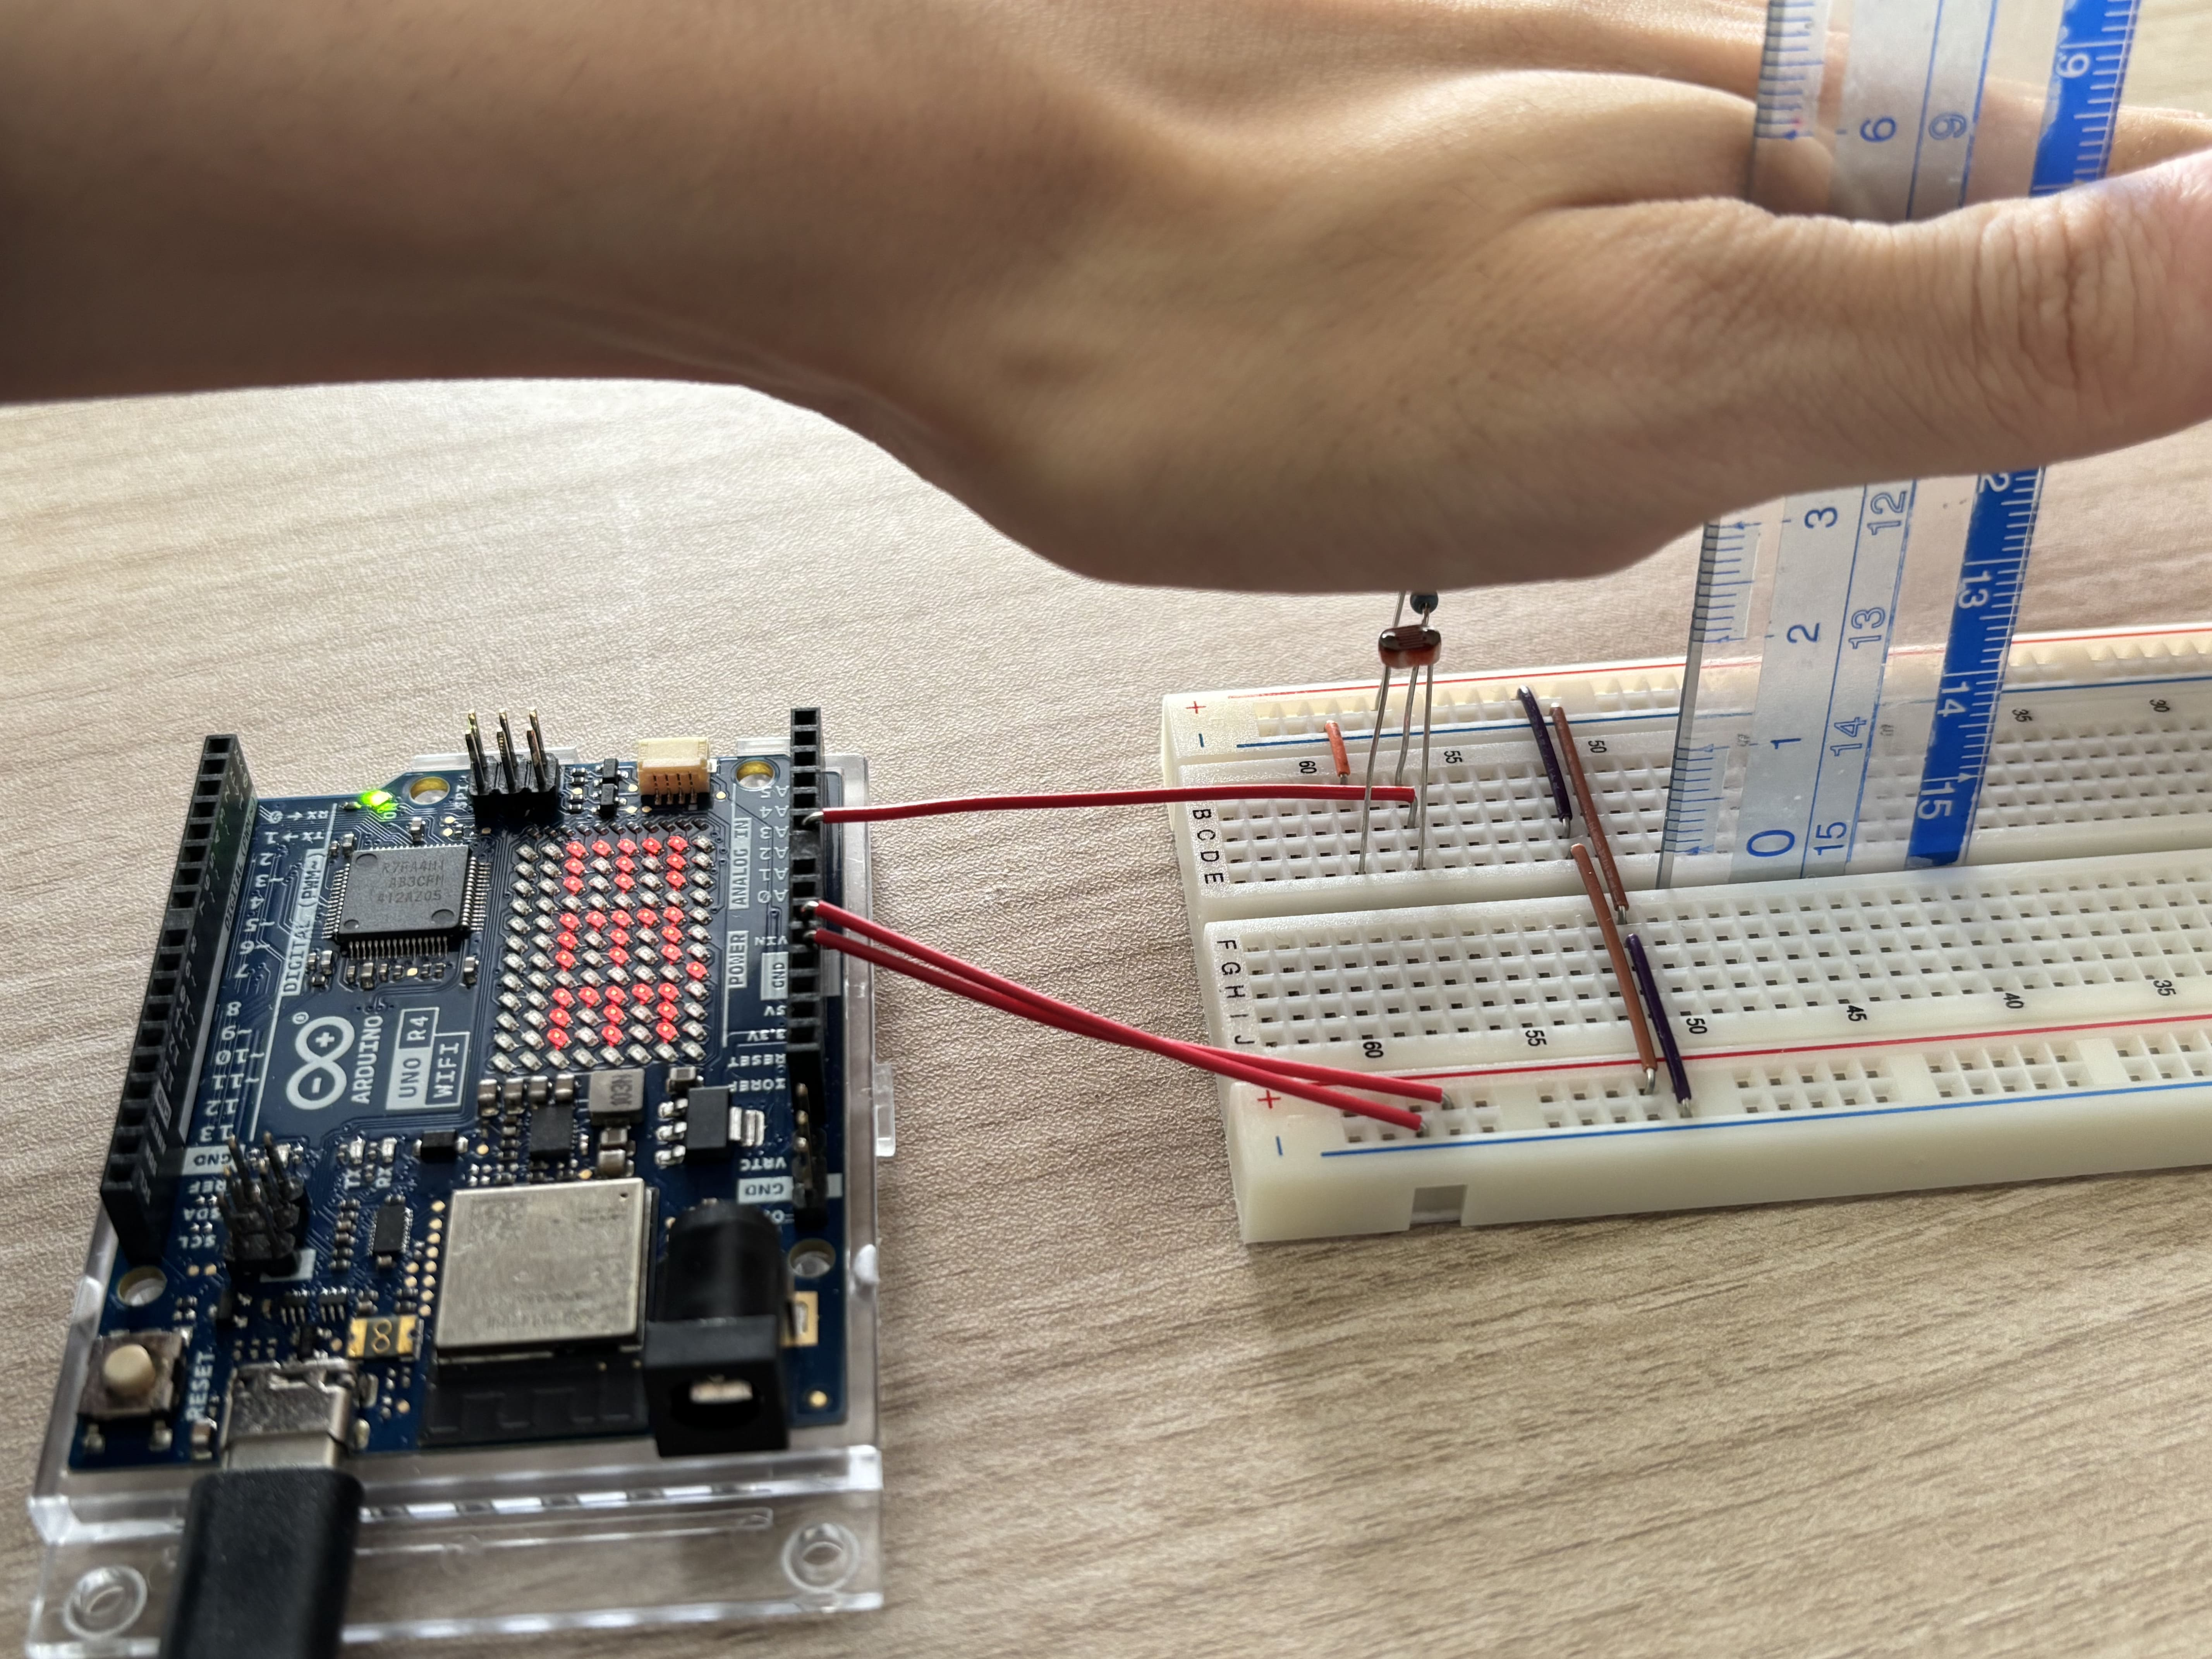
\includegraphics[width=0.8\linewidth]{fig_work_C/IMG_9293.jpg}
  \caption{CdSセルの上に定規を使用して手をかざす様子}
  \label{fig:C-2-keisoku}
\end{figure}
CSVファイルをもとに，Pythonを用いて作成した電圧値の変化を示すグラフで評価した．



\clearpage

\subsection{ワークC-3 時系列データの平滑化}


ワークC-2で取得した時系列データにはノイズが含まれるため，これを平滑化する処理の実装を行った．
本実習では，移動平均(Moving Average)および指数移動平均(Exponential Moving Average)の2種類の手法を用いて比較検証を行った．

移動平均は，直近$N$個のデータの単純平均を計算する手法である\cite{workC_MA}．
時刻$t$におけるデータ値を$x_t$とすると，移動平均値$y^{MA}_t$は式(\ref{eq:MA})で表される．
\begin{equation}
  y^{MA}_t = \frac{x_t + x_{t-1} + \dots + x_{t-N+1}}{N} \label{eq:MA}
\end{equation}
指数移動平均は，過去のデータほど重みを指数関数的に減少させ，直近のデータを重視する手法である\cite{workC_MA}．
平滑化係数を$\alpha = \frac{2}{N+1}$とすると，指数移動平均値$y^{EMA}_t$は式(\ref{eq:EMA})で表される．
\begin{equation}
  y^{EMA}_t = \alpha x_t + (1 - \alpha) y^{EMA}_{t-1} \label{eq:EMA}
\end{equation}

本実習では，ウィンドウサイズを$N=5$，$N=10$とし，移動平均の計算にはPythonのpandasライブラリのrolling()関数を用い，
指数移動平均の計算にはewm()関数を用いて計算を行った．
その後，元のデータと比較するグラフを作成して評価した．


\clearpage \section{結果} 
%実験から得られた結果について記述し，その中で読者の興味を引く結果がどれであり，それが何であるかを述べる．
%グラフや表にまとめるべきデータがあれば適切に図表として示すこと．
%本節の目的は図表を活用して要点を簡潔にまとめることであり，図表を文章にするのではない点に注意する．

\subsection{ワークC-1 LEDマトリクスの活用}
本実習では，フォトリフレクタと遮蔽物との距離を変化させ，電圧値との関係を示すグラフを作成した．
ArduinoのLEDマトリクスに表示された結果を表\ref{tab:C-1-result1}に示す．
\begin{table}[H]
  \caption{フォトリフレクタと遮蔽物との距離と電圧値}
  \centering
  \begin{tabular}{|c|c|c|c|c|c|c|c|c|c|c|}
    \hline
    距離 [cm] & 0.5 & 1.0 & 1.5 & 2.0 & 2.5 & 3.0 & 3.5 & 4.0 & 4.5 & 5.0 \\
    \hline
    電圧値 [V] & 2.20 & 3.37 & 4.11 & 4.42 & 4.57 & 4.70 & 4.74 & 4.76 & 4.78 & 4.79 \\
    \hline
  \end{tabular}
  \label{tab:C-1-result1}
\end{table}
表\ref{tab:C-1-result1}の数値から作成したグラフを図\ref{fig:C-1-result2}に示す．
\begin{figure}[H]
  \centering
  \includegraphics[width=0.6\linewidth]{../work/result_C1.png}
  \caption{フォトリフレクタと遮蔽物との距離と電圧値の関係}
  \label{fig:C-1-result2}
\end{figure}
横軸はフォトリフレクタと遮蔽物との距離 [cm]，縦軸は電圧 [V]を表している．
遮蔽物との距離が0.5 cmから2.5 cmの間では距離が離れるにつれて電圧値が急激に上昇し，
3.0 cm～5.0 cmでは電圧値の上昇が緩やかになり，約4.8 Vに収束する傾向が確認された．



\clearpage

\subsection{ワークC-2 ネットワークを介したデータの取得と分析}
CdSセルを用いて照度変化に伴う電圧の時間変化を測定した結果を図\ref{fig:C-2-result}に示す．
\begin{figure}[H]
  \centering
  \includegraphics[width=0.8\linewidth]{../work/result_C2.pdf}
  \caption{照度変化に伴う電圧の時間変化(生データ)}
  \label{fig:C-2-result}
\end{figure}
横軸は経過時間 [s]，縦軸は電圧 [V]を表している．
手をかざしていない状態(0～20秒，80～100秒)では約2.4 Vで安定しているが，
手をかざしてセンサへの光を遮ると電圧が上昇することが確認された．
また，手との距離が9.0 cm，6.0 cm，3.0 cmと近づくにつれて(20～80秒)，階段状に電圧値が増加する傾向が得られた．
一方で，電圧が一定となるべき区間においても，微小な電圧の振動(ノイズ)が観測された．



\subsection{ワークC-3 時系列データの平滑化}
ワークC-2で得られたデータに対し，ウィンドウサイズを$N=5$として移動平均および指数移動平均を適用した結果を図\ref{fig:C-3-result}に示す．
\begin{figure}[H]
  \centering
  \includegraphics[width=0.945\linewidth]{../work/result_C3.png}
  \caption{ウィンドウサイズを$N=5$とした平滑化手法による波形の違い}{(上：生データ，中：移動平均，下：指数移動平均)}
  \label{fig:C-3-result}
\end{figure}
上段は元の生データ，中段は移動平均，下段は指数移動平均の結果であり，横軸は経過時間 [s]，縦軸は電圧 [V]を表している．
いずれの手法においても，生データで見られた微細なノイズが低減され，波形が滑らかになっていることが確認できる．
特に，電圧が急激に変化するタイミング(手が移動するとき)において，移動平均と指数移動平均で生データに対する追従性に違いが見られた．

ウィンドウサイズを$N=10$として作成したグラフを図\ref{fig:C-3-result-N10}に示す．
\begin{figure}[H]
  \centering
  \includegraphics[width=0.92\linewidth]{../work/result_C3_N=10.png}
  \caption{ウィンドウサイズを$N=10$とした平滑化手法による波形の違い}{(上：移動平均，下：指数移動平均)}
  \label{fig:C-3-result-N10}
\end{figure}
上段は移動平均，下段は指数移動平均の結果であり，横軸は経過時間 [s]，縦軸は電圧 [V]を表している．



\clearpage \section{考察} 
%本ワークで得られた結果について考察する．
%例えば，以下のように記述する．

%（例）本ワーク○○では○○の結果が得られたが，これは理論値と比較して○○な結果である．これは○○が原因であると考えられる．

\subsection{ワークC-1 LEDマトリクスの活用}

本実習では，フォトリフレクタと遮蔽物との距離が電圧値に与える影響を検証した．
図\ref{fig:C-1-result2}に示すグラフでは，距離が0.5 cmから2.5 cmの間で電圧値が急上昇し，3.0 cm以降は約4.80 Vで収束する傾向が確認された．
この特有のグラフ形状は，光の強さが距離に応じて減衰する逆二乗の法則と\cite{workC_逆二乗の法則}，
センサ回路の電気的な特性を決定づけるオームの法則(式(\ref{eq:オームの法則}))によって説明できる\cite{workC_オームの法則}．
\begin{equation}
  V = I \times R \label{eq:オームの法則}
\end{equation}

まず，A0ピンで観測される電圧は，図\ref{fig:C-1-kairozu}に示す回路によって決定される．
この回路は，3.3 k$\Omega$の固定抵抗($R_2$)と，フォトリフレクタのフォトトランジスタ($R_P$)が直列に接続された分圧回路である\cite{workC_分圧回路}．
フォトトランジスタは，受光する光の強さに応じて抵抗($R_P$)が変化する可変抵抗として機能する．
A0ピンは，この$R_P$にかかる電圧($V_{out}$)を測定しており，その値はオームの法則に基づき，式(\ref{eq:A0電圧})の関係で表される．
\begin{equation}
  V_{out} = V_{CC} \times \frac{R_P}{R_2 + R_P} \label{eq:A0電圧}
\end{equation}

次に，受光する光の強さは逆二乗の法則に従う．
センサのLEDから放たれた赤外線は，遮蔽物に当たって反射し，フォトトランジスタに戻ってくる．
光は往復で距離の影響を受けるため，受光する光の強さは距離の二乗に反比例して急激に減少する．
この法則が，図\ref{fig:C-1-result2}のグラフのような形状を生み出す要因である．

これら2つの法則を組み合わせると，観測された図\ref{fig:C-1-result2}のグラフの傾向が説明できる．
遮蔽物が近い場合，反射光が強く，フォトトランジスタの抵抗値($R_P$)は低くなる．
分圧回路の特性により，$V_{out}$はGND側に引かれ，表\ref{tab:C-1-result1}では0.5 cmのとき2.20 Vという低い電圧となった．
遮蔽物を遠ざけると，逆二乗の法則に従い反射光が急激に減少し，$R_P$は高くなる．
これにより，$V_{out}$は分圧回路の特性に従って急激に上昇する．
そして，3.0 cm付近で反射光がほぼ0に近くなると，$R_P$は最大値に近くなり，それ以上はほとんど増加しなくなる．
その結果，$V_{out}$は電源電圧(5V)に近い約4.8 Vで収束したと考えられる．

以上の考察から，センサの出力電圧はフォトトランジスタが受光する赤外線の量によって決定されることがわかった．
本実習では距離を変数としたが，受光量は遮蔽物の反射率にも依存する．
したがって，本センサ回路の出力は，対象物との距離だけでなく，対象物の赤外線反射率にも強く関係していると考察できる．
この特性を利用し，一定の電圧を閾値とすることで，物体の有無を検知する非接触のスイッチへの応用が可能であると考えられる．




\subsection{ワークC-2 ネットワークを介したデータの取得と分析}

ワークC-2では，CdSセルを用いた回路の出力をネットワーク経由で連続的に測定し，光量の変化に伴う電圧値の変動を検証した．

まず，図\ref{fig:C-2-result}に示すように，手を近づけてセンサの照度が低下すると電圧値が上昇する結果が得られた．
この現象は，CdSセルの特性と，実験で用いた分圧回路の特性によって説明される．
CdSセルは，光のエネルギーを吸収することで内部の電子が増加し，電気抵抗が減少する性質を持つ\cite{workC_CdSセル}．
これにより，手を近づけてセンサへの入射光量が減少すると，CdSセルの内部抵抗($R_{CdS}$)が増加する．
図\ref{fig:C-2-kairozu}の回路は，固定抵抗($R_{fixed}$)と$R_{CdS}$が直列に接続された分圧回路であり，
A0ピンで測定される電圧($V_{out}$)は式(\ref{eq:A0電圧CdS})によって決定される\cite{workC_分圧回路}．
\begin{equation}
  V_{out} = V_{CC} \times \frac{R_{CdS}}{R_{fixed} + R_{CdS}} \label{eq:A0電圧CdS}
\end{equation}
この関係に基づき，照度低下によって$R_{CdS}$が増加すると，測定点($V_{out}$)にかかる電圧が上昇する．
CdSセルの性質により，手を近づけることによる照度低下は$R_{CdS}$の増加し，それに伴い分圧回路の特性によって$V_{out}$が上昇する．
その結果，図\ref{fig:C-2-result}のような電圧変化が観測されたと考察できる．

次に，20秒ごとの手の位置変更による大きな電圧変化のほかにも，電圧値に小さな変動が見られた．
この小さな変動の要因を考察する．
第一に，測定環境の照明の光のちらつきが，CdSセルでノイズとして検出された可能性が考えられる．
第二に，回路を流れる電流によるノイズや，Arduinoにおけるデジタル化に伴う誤差など，測定過程で生じるノイズが重畳している可能性がある．
第三に，一定の距離で手を静止させているつもりでも，測定者の微細な震えによって，センサ上を通過する光量がわずかに変動したこともノイズの一因として挙げられる．

続いて，手の位置を安定させる以外の方法で電圧値の小さな変動を低減する方法を検討する．
第一に，平滑化処理を適用する方法である．具体的には，移動平均や指数移動平均を計算することで，時系列データの高周波ノイズ成分を効果的に除去できる．
第二に，測定回路にコンデンサを追加する方法である．CdSセルにかかる電圧を測定しているA0ピンとGNDの間にコンデンサを接続することで，
RCローパスフィルタを構成し，高周波のノイズ成分をGND側にバイパスし，電圧の急激な変動を抑えることができる．
第三に，クライアント側のリクエスト間隔(1秒)はそのままとし，Arduino側のプログラムで複数回測定した平均値を返すように変更する方法である．
例えば，0.1秒ごとに10回測定し，その平均値を1秒のデータとしてクライアントに返すことで，瞬間的なノイズの影響を相殺し，低減することが可能となる．



\subsection{ワークC-3 時系列データの平滑化}
ワークC-3では，移動平均と指数移動平均によるノイズ除去効果を比較した．
図\ref{fig:C-3-result}より，両手法ともに高周波のノイズ成分を除去し，データの動向を捉えやすくする効果が確認された．

まず，手法間の違いとして，電圧が急激に変化する20秒付近，40秒付近，60秒付近，80秒付近での応答性に違いが見られた．
移動平均は過去$N$個のデータを均等に扱うため，急激な変化に対して値が追従するのに時間を要し，波形の立ち上がりが緩やかである傾向が強かった．
一方，指数移動平均は直近のデータを強く重要視するため，移動平均と比較して変化への反応が早く，変化に対してより忠実に追従していることがわかった．

次に，移動平均(式(\ref{eq:MA}))および指数移動平均(式(\ref{eq:EMA}))の両手法において，平滑化の結果に最も大きな影響を与えるパラメータはウィンドウサイズ($N$)である．
本実習では，ウィンドウサイズを$N=5$，$N=10$と設定し，それぞれ図\ref{fig:C-3-result}，図\ref{fig:C-3-result-N10}のグラフを作成した．
応答性の観点では$N=5$(図\ref{fig:C-3-result})，平滑化の観点では$N=10$(図\ref{fig:C-3-result-N10})が優れており，
グラフに対するウィンドウサイズの影響が明らかとなった．
移動平均では，$N$は平均を計算するために使用する直近のデータ数を表す．
$N$を大きくするほど，より多くの過去のデータを含めるため，波形はより滑らかになり，ノイズ除去効果は増大する．
しかし，同時に信号の急激な変化に対する遅延も大きくなり，信号の立ち上がりが鈍くなるという影響を与える．
指数移動平均では，$N$の値から式(\ref{eq:EMA_alpha})によって決定される平滑化係数$\alpha$によって制御される．
\begin{equation}
  \alpha = \frac{2}{N+1} \label{eq:EMA_alpha}
\end{equation}
$N$を大きくするほど$\alpha$は小さくなり，過去のデータに対する比率が相対的に増え，波形はより平滑化される．
しかし，移動平均と同様に，ノイズ除去と引き換えに変化への応答性は低下する．

今回のような状態が切り替わるデータの測定においては，ノイズを除去しつつも，状態変化のタイミングを正確に捉えることが重要である．
したがって，過去のデータの影響を長く引きずらず，変化への応答性が高い指数移動平均の方が，本システムの用途には適していると考察できる．



\clearpage

\section{おわりに} 
%ワークを通じて得られた知見や考察，目的の達成度などについて記述し，本ワークを総括する．
%単なる感想ではなく，客観的な総括を行うように注意すること．

本ワークでは，測定機器の出力機能および通信機能の開発を通じて，データの取得，表示，分析の一連のプロセスを習得することを目的とした．

まず，ワークC-1では，Arduinoに搭載されたLEDマトリクスを用いてセンサからの電圧値を小数点第2位まで表示するシステムを開発した．
これにより，マイコンボードの表示機能を実装する方法を理解した．

次に，ワークC-2では，ArduinoをWebサーバとして構築し，CdSセルで測定した環境光の強度データをネットワーク経由でクライアント側PCに送信するシステムを開発した．
これにより，測定機器が持つ通信機能と外部コンピュータとの連携を実現する方法を理解した．

最後に，ワークC-3では，取得された時系列データに含まれるノイズに対し，移動平均と指数移動平均の2種類の平滑化処理を施し，その結果を比較した．
これにより，指数移動平均が移動平均よりも急激な変化に対する応答性に優れていることを理解した．

以上の結果より，本ワークの目的であった「出力部および通信部の開発を通じて，データを取得・分析する方法を学ぶ」という目標は達成された．
物理量の測定から回路の特性に基づくデータ分析，そしてデータを平滑化するという一連のプロセスを実施することで，
感知システムとデータ処理についての理解を深めることができた．

\clearpage